\documentclass[11pt,t]{beamer}
\usepackage{color}
\usepackage{amsmath}
\usepackage{paralist}
\usepackage{setspace}
\usepackage{listings}
\usepackage{graphicx}
\usepackage{geometry}
\usepackage[utf8]{inputenc}
\usepackage{etex} % Avoid an error due to a lack of registers
\usepackage[ngerman]{babel} % Defines the language of macros as well
% Desired Packages
%\usepackage[pdftex]{graphicx}
\usepackage[utf8]{inputenc}
\usepackage{amsmath}
\usepackage{amssymb}
\usepackage{lastpage}
\usepackage{listings}
\usepackage{caption}
\usepackage{xy}
\usepackage{microtype}
\usepackage{lmodern, hfoldsty}
\usepackage{ellipsis}
\usepackage{tabularx}
\usepackage{beamerthemeshadow}
\usepackage{nameref}
\usepackage{hyperref}
\usepackage{subfig}
\usepackage[absolute,overlay]{textpos}
\setlength{\TPHorizModule}{\paperwidth}
\setlength{\TPHorizModule}{\paperheight}

% Further Configurations
\newcommand{\Fat}[1]{{\large \bf \textcolor{cdc_Blue}{#1}}}
\renewcommand\rmdefault{pmy}            		% Activate Myriad Font
\definecolor{Gray}{rgb}{0.5, 0.5, 0.5}  		% Define light color
\definecolor{HighlightRed}{rgb}{0.6, 0.0, 0.0}  % Define light highlighting color
\graphicspath{{images/}}
\usetheme{UniOldbg}                     		% The main thing: our theme


\newcommand*\conj[1]{\bar{#1}}
\newcommand*\mean[1]{\overline{#1}}

\title[Theoretische Ozeanographie]{Turbulenzmodelle}
\author[Florian Börgel]{Florian Börgel}
\date{\today}
\semester{Sommersemester 2016}
\institute{Universität Oldenburg}


\AtBeginSection[]{
	\frame{
		\frametitle{Inhaltsverzeichnis}
		\tableofcontents[currentsection]
	}
}
\begin{document}

\frame{\titlepage}
\frame{\frametitle{Gliederung}\tableofcontents}

%%%%%%%%%%%% Start of content %%%%%%%%%%%% 
\section{Direct Numerical Simulation}
\begin{frame}
\frametitle{DNS}
\begin{figure}
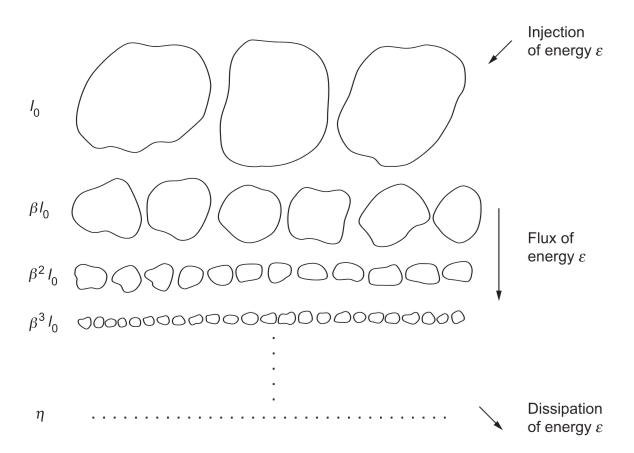
\includegraphics[width=0.8\linewidth]{images/cascade.png}
			\caption{Energiekaskade}
\end{figure}
\end{frame}
\begin{frame}
	\frametitle{DNS}
Die größten Wirbel in der Strömung haben den größten Anteil an dem Transport von Bewegung und Energie. Die größte Skala wird also durch 
\begin{equation}
L
\end{equation}
festgelegt. Die Größe der kleinsten Skala wird durch die Viskosität definiert. (Kinetische Energie wird in Wärme dissipiert)
\begin{equation}
\eta = (\frac{\nu^3}{\epsilon})^{1/4}
\end{equation}
\hspace{1cm}$\epsilon$ - Dissipationsrate\\
\hspace{1cm}$\nu$ - Viskosität
\end{frame}


\begin{frame}
	\frametitle{Turbulente Längenskalen}
\begin{equation}
\epsilon\thicksim \frac{U^3}{L}
\end{equation}
\begin{equation}
\eta = \frac{\nu^3 * L}{U^3}
\end{equation}
Für $1D$ gilt also:
\begin{equation}
\frac{L}{\eta} = Re^{3/4} 
\end{equation}

\vspace{0.5cm}
\textit{aktueller Stand:} $8000*8000*8000$

\begin{quote}
de Bruyn Kops, S.M., 2015. Classical scaling and intermittency in
strongly stratified Boussinesq turbulence. Journal of Fluid Mechanics
775, 436–463. doi:10.1017/jfm.2015.274
\end{quote}
\end{frame}


\section{Reynold-Averaged Navier-Stokes Equation}


\begin{frame}
	\frametitle{Vereinfachungen}
\begin{equation}
\frac{\partial}{\partial t} = \partial_t, \hspace{0.3 cm}\frac{\partial}{\partial x} = \partial_x,\hspace{0.3 cm} \frac{\partial}{\partial x_i} = \partial_i
\end{equation}
\begin{equation}
\sum_{j=x,y,z}u_j\partial_j = u_j\partial_j
\end{equation}
\end{frame}

\begin{frame}
\frametitle{Reynolds-Averaged Navier-Stokes Equations}
NSE:
\begin{equation}
\partial_t u_i + \partial_j u_ju_i = -\frac{1}{\rho}\partial_i p + \nu\partial^2_j u_i
\end{equation}
gemittelte Gleichung:
\begin{equation}
\partial_t \overline{u_i} + \partial_j \overline{u_ju_i} = -\frac{1}{\rho}\partial_i \overline{p} + \nu\partial^2_j \overline{u_i}
\end{equation}
Reynolds-Zerlegung:
\begin{equation}
u = \overline{u} + u'
\end{equation}
\end{frame}

\begin{frame}
Einsetzen:
\begin{align}
\partial_t \overline{\bar{u_i}} + \partial_t \overline{u_i^{'}}+ \partial_j (\overline{\bar{u_i}*\bar{u_j}} + \overline{\bar{u_i}*u_j^{'}} + \overline{u_i^{'}*\bar{u_j}} + \overline{u_i^{'}*u_j^{'}}) \\
= - \frac{1}{\rho}*\partial_i*(\overline{\bar{p}+p^{'}}) + \nu*\partial_j^2  (\overline{\bar{u_i}+u_i^{'}})
\end{align}
Es gilt $\overline{u^{'}},\overline{p^{'}} = 0$, daher:
\begin{align}
\partial_t \bar{u_i} + \partial_j (\overline{u_iu_j}+{\color{red}\overline{u_i^{'}u_j{'}}}) = - \frac{1}{\rho} \partial_i \bar{p}+\nu*\partial_j^2\bar{u_i}
\end{align}
\begin{align}
\partial_tu_i+\partial_j(\mean{u_i^{'}u_j^{'}}) = - \frac{1}{\rho} \partial_i \bar{p}+\partial_j(\nu\partial_j\bar{u_i}-{\color{red}\overline{u_i^{'}u_j{'}}})
\end{align}
$\tau_{ij,turb} = -\rho\overline{u_i^{'}u_j{'}}$ = Reynold-Stress-Tensor
\end{frame}
\section{Schließungs Problem der Turbulenz}
\begin{frame}
Wie kann man den Reynold-Stress-Term beschreiben? Auch als Transport-Gleichung?
\begin{align*}
&\partial_t\overline{u_i^{'}u_j{'}}+u_a\partial_a\overline{u_i^{'}u_j{'}} =\\& -\overline{u_j^{'}u_a{'}}\partial_a\bar{u_i}
-\overline{u_j^{'}u_a{'}}\partial_a\overline{u_j}-\partial_a\overline{u_i^{'}u_j{'}u_a^{'}} \\&- \frac{1}{\rho}(\partial_i\overline{u_j^{'}p^{'}}+\partial_j\overline{u_i^{'}p^{'}})+\frac{1}{\rho}(\overline{p^{'}\partial_iu_j^{'}}+\overline{p^{'}\partial_ju_i^{'}})+\nu(\partial_a^{2}\overline{u_j^{'}u_i^{'}}-2\overline{\partial_au_i^{'}\partial_au_j^{'}})
\end{align*}
Umformen:
\begin{align*}
&\partial_t\overline{u_i^{'}u_j{'}}+u_a\partial_a\overline{u_i^{'}u_j{'}} =\\& -\overline{u_j^{'}u_a{'}}\partial_a\bar{u_i}
-\overline{u_i^{'}u_a{'}}\partial_a\overline{u_j}- 2\nu\overline{\partial_au_i^{'}\partial_au_j^{'}}\\&+\overline{\frac{p^{'}}{\rho}(\partial_iu_j^{'}+\partial_ju_i^{'})}+\partial_a (\nu\partial_a\overline{u_j^{'}u_i^{'}} -\overline{u_i^{'}u_j{'}u_a^{'}}-\frac{1}{\rho}(\partial_i\overline{u_j^{'}p^{'}}+\partial_j\overline{u_i^{'}p^{'}}))
\end{align*}
\end{frame}
\section{Transport Energy Equation}
\begin{frame}
Mit dieser Transportgleichung, kann nun die Transportgleichung für die turbulente kinetische Energie aufgestellt werden.\\
Diese ist definiert als: $\mean{k} = \frac{1}{2}\mean{u_j^{'2}}$
Setzt man nun in der Transport-Gleichung: i = j erhält man:
\begin{align*}
2\partial_t \mean{k} + 2\mean{u_a}\partial_a \mean{k} = -2\overline{u_j^{'}u_a{'}}\partial_a\bar{u_j}
- 2\nu\overline{\partial_au_j^{'}\partial_au_j^{'}}\\+\overline{\frac{p^{'}}{\rho}(\partial_ju_j^{'}+\partial_ju_j^{'})}+\partial_a (2\nu\partial_a\overline{k} -2\overline{k u_a^{'}}-\frac{2}{\rho}(\partial_j\overline{u_j^{'}p^{'}}))
\end{align*}
\begin{align*}
\partial_i u_i = 0\\
\overline{\frac{p^{'}}{\rho}(\partial_ju_j^{'}+\partial_ju_j^{'})} = 0 \\
\end{align*}
\end{frame}
\begin{frame}
\begin{align*}
&\underbrace{\partial_t \mean{k}} + \underbrace{\mean{u_k}\partial_k \mean{k}} = -\underbrace{\overline{u_j^{'}u_a{'}}\partial_a\bar{u_j}}- \underbrace{\bar{\epsilon}} - \underbrace{\partial_a (\nu\partial_a\overline{k} -\overline{k u_a^{'}}-\frac{1}{\rho}(\partial_j\overline{u_j^{'}p^{'}}))}\\
&\hspace{0.3cm}L \hspace{1.1cm}C \hspace{1.8cm}P\hspace{1.1cm} DS \hspace{2.3cm}TS\\
\end{align*}
\end{frame}

\section{Turbulenz-Modelle}
\begin{frame}
\frametitle{Turbulenz-Modelle}
Die bisherigen Gleichungen sind nicht geschlossen. Deshalb wird der Reynold-Stress-Tensor modelliert.
\begin{align*}
\overline{u_i^{'}u_j{'}} = \nu_t(\partial_j \bar{u_i} + \partial_i \bar{u_j})-\frac{2}{3}\mean{k}\delta_{ij}
\end{align*}
$\nu_t$ ist die Wirbelviskosität (Analog zur Idee vom molekularen shear stress) 
\end{frame}
\begin{frame}
\frametitle{Turbulenz-Modelle}
Es gibt verschiedene Modelle um das Problem zu lösen. Hier Wirbelviskosität-Modelle\\
\begin{tabular}{l l l}
&\\
Prandtl mixing-length: & $\nu_t = l_m^2\overline{S_{ij}}$& algebraisch\\
&\\
Prandtl-Kolmogorov: &$\nu_t = C_\mu l_{pk}\sqrt{k}$& 1-Gleichungs-Modell\\
&\\
k-$\epsilon$-Modell & $\nu_t = C_\mu \frac{k^2}{\epsilon}$& 2-Gleichungs-Modell\\
\end{tabular}
\end{frame}
\begin{frame}
\frametitle{Prandtl mixing-length}:
\begin{equation}
\nu_t = l_m^2\overline{S_{ij}},\hspace{0.5cm}\overline{S_{ij}} = \frac{1}{2}(\partial_i \overline{u_j} + \partial_j \overline{u_i})
\end{equation}
\begin{itemize}
\item[•]Based on dimensional analysis
\item[•]Empirical methods for determining $l_m$
\item[•]Assumption $l_m$ = const.
\end{itemize}
\end{frame}

\section{k-$\epsilon$ Model}

\begin{frame}
Setzen wir diese Beziehung einmal ein:
\begin{align*}
P &= -\mean{u_i^{'}u_j^{'}}\partial_j\mean{u_i}\\
P &= (\nu_t(\partial_j \bar{u_i} + \partial_i \bar{u_j})-\frac{2}{3}\mean{k}\delta_{ij})\partial_j\mean{u_i}\\
TS &= \partial_a (\nu\partial_a\overline{k} -\overline{k u_a^{'}}-\frac{1}{\rho}(\partial_j\overline{u_j^{'}p^{'}}))\\
TS &= \partial_i(\frac{\nu_t}{Pr_k} \partial_i \mean{k})
\end{align*}
\end{frame}

\begin{frame}
\frametitle{k-$\epsilon$-Modell}
\begin{align*}
\nu_t &= C_\mu \frac{k^2}{\epsilon}\\
\partial_t \mean{k}+ \mean{u_i}\partial_i \mean{k} &= P_k - \mean{\epsilon} + \partial_i(\frac{\nu_t}{Pr_k} \partial_i \mean{k})\\
\partial_t \mean{\epsilon}+ \mean{u_i}\partial_i \mean{\epsilon} &= \partial_i(\frac{\nu_t}{Pr_k} \partial_i \mean{k}) + \frac{\epsilon}{\mean{k}}(c_{\epsilon 1}P_{k}+c_{\epsilon 2}\mean{\epsilon})
\end{align*}
\end{frame}

\section{Einsatz in der Ozeanographie}
\begin{frame}
\frametitle{Einsatz in der Ozeanographie}
Wie werden dieses Ideen jetzt in der Ozeanographie eingesetzt?
\begin{quote}
'two-equation turbulence closure models have emerged as work horses for vertical turbulent fluxes' - Die Küste, 81 (2014, 72)
\end{quote}
\\
$\Rightarrow$ k-$\epsilon$ Modell\\
\vspace{1cm}
Für die vertikalen turbulenten Strömungen gibt es bereits Schließungsmodelle.
Bei horizontalen wird die Diffusion entweder ignoriert oder eine konstante horizontale Viskosität gewählt.
\end{frame}
\begin{frame}
\frametitle{Ozeanmodellierung}
GETM  (General Estuarine Transport Model): 3D Transportmodell für Ozeane\\
\pause
Kopplung mit $\Rightarrow$ GOTM (General Ocean Turbulence Modell)

\end{frame}

%%%%%%%%%%%% End  %%%%%%%%%%%%

\section*{Ende}

	\begin{frame}
		\frametitle{Ende}
		\begin{center}
			\Large \textbf{Vielen Dank für Ihre Aufmerksamkeit!}\\
			\large \textbf{Haben Sie Fragen?}\\
		\end{center}
	\end{frame}
	
	% Black frame to separte appendix
	\setbeamercolor{background canvas}{bg=black}
	\begin{frame}[plain]
	\end{frame}
	\setbeamercolor{background canvas}{bg=white}

%%%%%%%%%%%% Start of appendix %%%%%%%%%%%% 

%%%%%%%%%%%% End of appendix %%%%%%%%%%%%

\end{document}